

\begin{definition}
\label{def:invariant}
Consider a 1d-family of $N-$periodic orbits of an elliptic billiard.  A quantity (function) is called invariant when it is constant over the family. 
\end{definition}

A classical invariant of the family of  billiard $N-$periodic orbits $\{P_1(u),\ldots, P_N(u)\}$ is the length 
\[ L(u)=\sum_{i=1}^N |P_{i+1}(u)-P_i(u)|.\]

The other invariant  is the Joachimstall's constant which is given
\[J_i(u)= \big\langle A P_i(u),\frac{P_{i+1}(u)-P_{i }(u)}{ |P_{i+1}(u)-P_{i }(u)|}\big\rangle.\]

\begin{theorem}\label{thm:soma_cossenos_N}
The sum of cosines of elliptic billiard N-periodic cosines is invariant for all N and given by $J L - N$.
\end{theorem}

\section{Proof for \torp{$N=3$}{N=3}}

This section is based in 
\cite{reznik2020-intelligencer, garcia2020-new-properties}.

Let $r(t)$ and $R(t)$ be the radius of the incircle and circumcircle aof 3-periodic billiard orbit $\mathcal{P}_3(t)=\{p_1(t),p_2(t),p_3(t)\}$, respectively.

\begin{theorem}
\label{thm:05-rovR-invariant}
$r/R$ is invariant over the 3-periodic orbit family and given by
\begin{equation}
\label{eqn:05-rovR-3periodic}
\frac{r}{R}=\frac{2 (\delta-b^2)(a^2-\delta)}{(a^2-b^2)^2}.
\end{equation}
\end{theorem}
\begin{proof}
Let $r$ and $R$ be the radius of the incircle and circumcircle, respectively. For any triangle \cite{coxeter67} we have

\begin{equation*}
 rR=\frac{s_1s_2s_3}{2 L}, 
\end{equation*}

\noindent where $L=s_1+s_2+s_3$ is the perimeter, constant for 3-periodic orbits. %; see \cref{eqn:perimeter}. Therefore,

\begin{equation}
\frac{r}{R}=\frac{1}{2L} \frac{s_1s_2s_3}{R^2}\cdot
\label{eqn:05-rovR-cas}
\end{equation}

Next, with $P_1=(a,0)$, obtain a {\em candidate} expression for $r/R$. This yields \cref{eqn:05-rovR-3periodic} exactly. Using explicit expressions for orbit vertices (see) %\cref{app:orbit-vertices}),
derive an expression for the square of the right-hand side of \cref{eqn:05-rovR-cas} as a function of $x_1$ and subtract from it the square of \cref{eqn:rovR}. It can be shown $\left(s_1s_2s_3/R^2\right)^2$ is rational on $x_1$ \cite{garcia2020-ellipses}. For simplification, use $R=s_1 s_2 s_3/(4A)$, where $A$ is the triangle area. With a computer algebra system (CAS), show said difference is identically zero for all $x_1\in(-a,a)$.
\end{proof}

\begin{corollary}
\[\cos\theta_1(t)+\cos\theta_2(t)+\cos\theta_3(t)=1+\frac{r(t)}{R(t)} \]
is invariant over the 3-periodic orbit family.
\end{corollary}

\begin{proof}
The relation stated is valid for any triangle. Therefore the result follows directly from Theorem \ref{thm:05-rovR-invariant}.
\end{proof}
\section{Case of \torp{$N=4$}{N=4}}

\begin{theorem}\label{thm:c4} Let $\mathcal{P}_4(t)=\{p_1(t),p_2(t),
p_3(t),p_4(t)\}$ 
be the family of 4-periodic billiard orbits.
Then,
\[\sum_{i=1}^4\cos \theta_i(t)=0\]
\label{th:soma_4cossenos}
\end{theorem}

\begin{proof}
If the orbit is simple it is a parallelogram and the result follows.
When the orbit is self intersected it is inscribed in a circle    and therefore the opposite angles are supplementary and so the result follows.
\end{proof}

\section{Proof for all \torp{$N$}{N} via Linear Algebra}
This section is based in   \cite{akopyan2020-invariants}.
Consider the ellipse $\E$ defined by $\langle Ap,p\rangle=1$, 
where $A$ is a diagonal matrix 
\[A=\left(\begin{matrix} \frac{1}{a^2} &0\\
0&\frac{1}{b^2}\end{matrix}\right)\]
Let also $p_i^*=Ap_i$, 
We have that $p_i^*$ is a normal vector to the ellipse $\E$ at $p_i$ and $\langle p_i,p_i^*\rangle=1.$
\begin{proposition}
The function
\[ J(p,u)=-\langle p^*,u\rangle\]
is invariant under the billiard map $T(p,u)=(q,v).$
\end{proposition}

 
\begin{proof}
See \cref{prop:appA-joachim}.
\end{proof}

\begin{theorem} \label{th:soma_cossenos} Let   $\mathcal{P}_N=\{p_1,\ldots, p_N\}$ be a $N-$periodic orbit of an elliptic billiard $\E$ with internal angle $\theta_i$ at the vertex $p_i$. Then,
\[\sum_{i=1}^{N}\cos\theta_i=JL-N\]
\end{theorem}


\begin{proof} Consider a $N-$periodic orbit $\mathcal{P}_n=\{p_1,\ldots, p_N\}$ and let $u_i$ be the unitary vector defined by 
\[u_i=\frac{p_{i+1}-p_i}{|p_{i+1}-p_i|.}\]

Let $p_i^*=Ap_i$. We have that $p_i^*$ is a normal vector to the ellipse $\E$ at $p_i$ and $\langle p_i,p_i^*\rangle=1.$

Then, the polygonal orbit $\mathcal{P}_n$ has perimeter $L$ given by 
\begin{align*}
    L&= \sum \langle p_{i+1}-p_i, u_i\rangle=\sum \langle p_{i} , u_{i-1}\rangle-\sum \langle  p_i, u_i\rangle=\sum \langle p_i, u_{i-1}-u_{i}\rangle\\
\end{align*}
By the reflection law we have that:
\[u_{i-1}-u_i=2\sin\left(\frac{\pi-\theta_i}{2}\right)\frac{p_i^*}{|p_i^*|}=2\cos\left(\frac{\theta_i}{2}\right)\frac{p_i^*}{|p_i^*|}\]

Also,

\[J=-\langle u_i,p_i^* \rangle=-\cos\left(\pi-\frac{\theta_i}{2}\right)|p_i^*|=\cos\left(\frac{\theta_i}{2}\right)|p_i^*|\]

Since $\langle p_i,p_i^*\rangle=1$ and $J$ is invariant it follows that
\begin{align*}
JL&=\sum \cos\left(\frac{\theta_i}{2}\right)|p_i^*|\langle p_i, u_{i-1}-u_{i}\rangle=
\sum \cos\left(\frac{\theta_i}{2}\right)|p_i^*|\langle p_i,2\cos\left(\frac{\theta_i}{2}\right)\frac{p_i^*}{|p_i^*|}\rangle\\
&=\sum 2\cos^2\left( \frac{\theta_i}{2}\right)\langle |p_i^*|p_i, \frac{p_i^*}{|p_i^*|}\rangle=\sum (1+\cos\theta_i)= N+\sum\cos\theta_i
%
\end{align*}
\end{proof}


%\section{Proof for all \torp{$N$}{N} via Liouville}
 \section{  Cosine sum of central angles of \torp{$N$}{N}-gons }
 
This section is based in \cite{akopyan2020-invariants} and
\cite{bialy2020-invariants}. 
%The result will be obtained from the Liouville's theorem.
In this section we will consider the Poncelet pair given by a unit circle $\mathcal{C}$ and an ellipse $\E$, both centered at $0$ and 
$\E\subset \mathcal{C}.$

\begin{theorem}
Consider a Poncelet orbit $\{p_1,p_2,\ldots, p_N\}$ inscribed in a circle $\mathcal{C}$ and circumscribed in an ellipse $
\mathcal{E}$, both centered at $0.$
Then 
\[\sum_{i=1}^N \cos \alpha_i= \sum_{i=1}^N \cos\angle p_{i-1}0p_{i}\] is constant in the 1-parameter family of Poncelet $N$-gons.
\label{th:somacossenos_liouville}
\end{theorem}
\begin{figure}
    \centering
    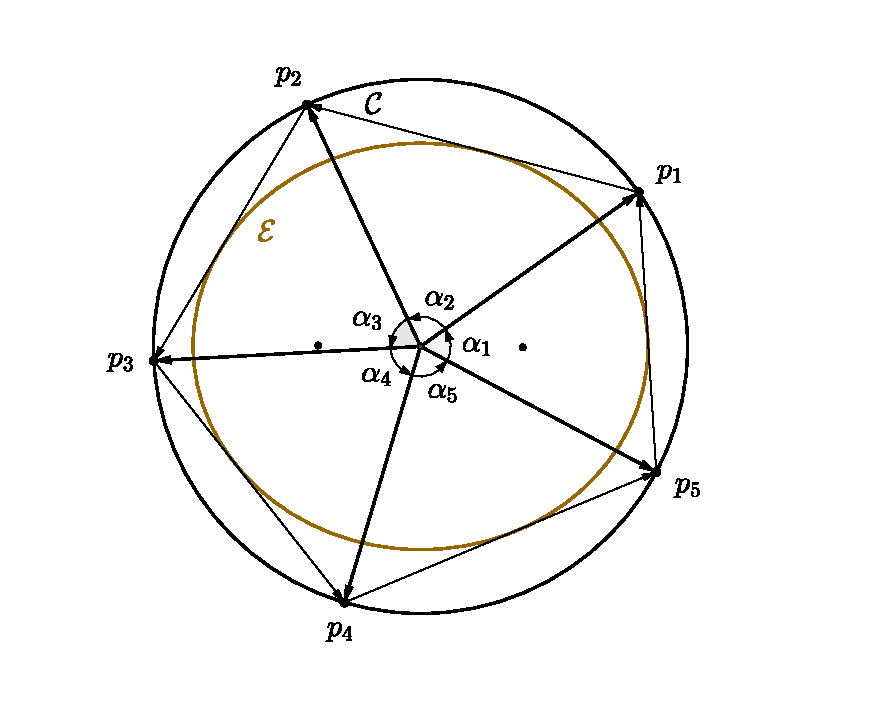
\includegraphics[scale=0.8]{pics-05-120-orbita5_C_E.pdf}
    \caption{Poncelet 5-periodic orbit.}
    \label{fig:orb5_poncelet}
\end{figure}
\begin{proof} The idea is to complexify the problem and show that the sum is bounded.  

Consider the rational parametrization 
\[ p(t)=\left(\frac{2t}{t^2+1},\frac{t^2-1}{t^2+1}\right),\] 
of the conic $x^2+y^2=1 $ with $t\in\mathbb{C}$.

We have that

\[S_N=\sum_{i=1}^N \cos\angle p_{i-1}0p_{i}=\langle p_{i-1}, p_i\rangle. \]

The sum $S_N$ can be unbounded only when the complexified orbit contains   points  at infinity which are given by $p(I)$ and $p(-I)$. Here $I$ is the complex number with $I^2=-1.$

\noindent {\bf Claim:} If $p(I)$ is a vertex of a Poncelet polygon, then the adjacent (neighboring) vertices to $p(I)$, say $a(I)$ and $b(I)$, are opposite in $\Cm.$

The complex lines $p(I)a(I)$ and $p(I)b(I)$ are tangent to the complex conic $\E$ and are parallel, therefore the tangency points of these lines with $\E$ are symmetric with respect to $O$. Hence their intersection points with $\Cm$ are also symmetric (the point $p(I)$ is invariant under a reflection in $O$, given by the Möbius map $M(t)=-1/t$).

 \noindent {\bf Claim:} For any finite point $q$   on $\Cm$, it follows that
 \[ \langle  q, a(I)\rangle +\langle q, b(I)\rangle  =  \langle  q, a(I)+b(I)     \rangle=\langle q,0\rangle=
0.\]
 Now, consider the point $p(t +I)$ with $t$  tending to zero and its adjacent (neighboring) vertices
$a(I +t)$ and $ b(I +t)$ of the Poncelet polygon. Notice that $   p(t + I) $ tends to infinity as
$0(1/t)$, while $a(t + I), b(t + I)$ tend to their limits $a(I), b(I)$ linearly. Furthermore,
due to the symmetry, as $t$ goes to zero, the linear in $t$ terms are vectors with the same
absolute value and opposite directions:
\[a(t+I)=a(I)+\mathbf{k} t+O_1(t^2),\;\;b(t+I)=-a(I)-\mathbf{k} t+O_2(t^2).\]

\noindent Therefore, for small $t$ we have:
\begin{align*}
\langle p(t + I ), a(t + I )\rangle + \langle p(t + I ), b(t + I )\rangle & = \langle p(t + I ), a(t + I ) + b(t + I )\rangle\\
&= \langle 0(1/t),0(t^2)\rangle = 0(t).
\end{align*}
Then,
 \[ \langle  p(I), a(I)\rangle +\langle p(I), b(I)\rangle  =   
0.\]
So the function $S_N$ is bounded and by Liouville's theorem it is constant.
\end{proof}

\begin{example} In the case $N=3$ we have that
\begin{align*}
p(I)&= \infty , \; a(I)=[{ {\frac {a}{\sqrt {2\,a-1}}}},     {\frac {I(a-1)}{\sqrt {2\,a-1}}}],\;\; b(I)=-a(I)\\
p(I+t)&=\frac{1}{t} -{\frac {I}{2}}+{\frac{1}{4}}t+O \left( {t}^{2} \right)  \\
a(I+t)&= { {\frac {a}{\sqrt {2\,a-1}}}}+{\frac { \left( a-1 \right) ^{2}a}{2\,
a-1}}t+O \left( {t}^{2} \right), \; b(I+t)=-a(I+t)+O(t^2)
%
\end{align*}
\end{example}
\begin{remark}
The internal angles $\alpha_i$ of the Poncelet polygon $\{p_1,p_2,\ldots, p_N\}$ satisfy
$\alpha_i=\pi-\angle p_{i-1}0p_i$ and therefore the \cref{th:somacossenos_liouville} is equivalent to \cref{th:soma_cossenos}.
\end{remark}

\begin{proposition} Consider the Poncelet pair $x^2+y^2=1$ and $x^2/a^2+y^2/(1-a)^2=1$, with $0<a<1.$
Then \[\sum_{i=1}^3\cos\theta_i=2a^2-2a-1.\]
\end{proposition}

\begin{proof} In this case a 3-periodic orbit is given
by $p_1=(x_1,y_1)$
\begin{align*}
    p_2&=\left[\frac{ a(-x_1(a - 1)^2 + y_1\Delta } { (1-2a)x_1^2 + a^2  }, \frac{(a - 1)(a^2y_1 + x_1\Delta) }{  (1-2a)x_1^2 + a^2 }
\right]\\
p_3&=\left[-\frac{ a(x_1(a - 1)^2 + y_1\Delta } { (1-2a)x_1^2 + a^2  }, \frac{(a - 1)(a^2y_1 - x_1\Delta) }{  (1-2a)x_1^2 + a^2 }
\right]\\
\Delta&= \sqrt{a^3(2-a  ) + x_1^2(1-2a )}
\end{align*}
 Computing the cosines the result follows by straightforward calculations with  help of CAS.
\end{proof}
\section{Average Cosine Sum with Spatial Integrals}

%\section{Future Work}

In \cite{reznik2021-fifty-invariants} we provide a list of invariants, many conjectured.
